\section{Methodology} \locallabel{sec:methodology}

In this section we describe the classes in our study, the concept of a feedback
delay, and provide some details on our system architecture.

\subsection{Classes}

\begin{figure}[!t]
\centering 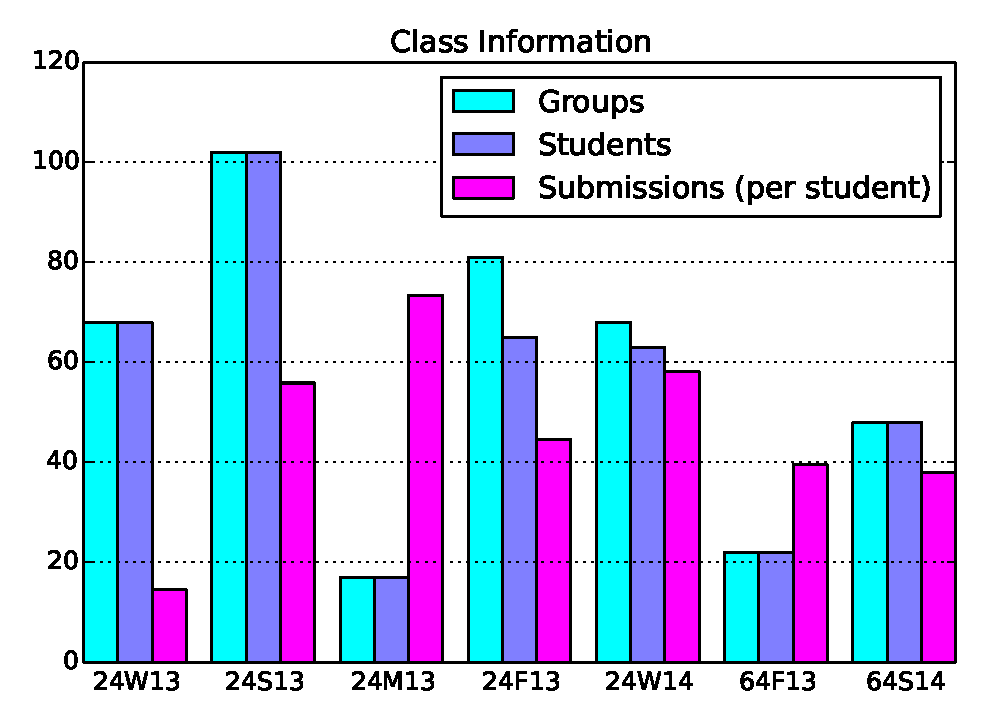
\includegraphics[width=3.3in]{graphs/Class_Information.eps}
\caption{Visualizes the number of groups, students, and average number of
  submissions by student for each of the seven classes in the study.}
\locallabel{fig:class_info}
\end{figure}

Our study involves multiple instances of two courses. The first course,
\emph{CS24}, is the second required course in UCSB's lower division Computer
Science curriculum that builds upon student's prior knowledge of \emph{C} in
order to educate them on basic data structures, and basic object oriented
programming in \emph{C++}. The second course, \emph{CS64}, is a lower division
computer architecture course that educates students on assembly programming and
the basics of computer architecture including digital design. In total, there
are five instances of \emph{CS24}, and two instances of \emph{CS64} represented
in this study. A single instructor taught \cm[24]{13} and \cf[24]{13}, and the
remainder were taught by another instructor. All classes were taught during a
10-week quarter including the summer instance.

Figure~\localref{fig:class_info} shows the relevant information for each of the
classes in this study. The purple bars indicate the number of students who
provided consent in each of the classes. The cyan bars indicate the number of
unique groups to make submissions on the class's assignments, and the pink bars
indicate the average number of submissions made by each student. Submissions
for non-programming assignments are excluded.

We distinguish between students and groups because the submission system
supports an instructor defined group size on a per assignment basis allowing
students to manually form groups for such assignments. Where groups are
concerned, only submissions for which we have the consent of all group members
are included. This grouping functionality was only introduced in September
2014, and thus it was only utilized in \cf[24]{13} and \cw[24]{14}. In those
classes, the groups did not remain consistent as students could change
partners, or chose to work independently (considered a single student group)
from assignment to assignment.

The average number of submissions is low for \cw[24]{13} due to only using the
submission system for half of the quarter. The average number of submissions
per student for \cm[24]{13} is relatively high due to students making
post-deadline submissions as discussed in Section~\localref{sec:deadline}.


\subsection{Feedback Delay} \locallabel{sec:delay}
The purpose of the real-time feedback system is simply to provide feedback to
the students so they may iteratively achieve mastery of an assignment. The
usage of such systems has positive side effects including reducing assessment
time while increasing assessment equitability. However, as many have previously
observed, student usage of such systems may result in dependency upon the
system. This dependency could inhibit students from expanding their knowledge
of the compilation, execution, testing, and debugging processes.

Web-CAT ensures students develop testing skills by requiring students to submit
test cases along with their code~\cite{Edwards:2003:RCS:949344.949390}. While
this approach appears successful to help students develop testing skills, such
an approach would require a change to our lower-division curriculum. In order
to encourage students to start assignments earlier, Marmoset introduced the
concept of limited release tokens where feedback from a subset of tests could
only be received a few times a day. In theory, the release token approach
should also discourage dependency on the system; however, in practice \spacco{}
indicated that very few students took advantage of the release
tokens~\cite{Spacco:2013:TIP:2462476.2465594}.

We built our system in order to take an alternative approach that could
transparently be utilized by UCSB's computer science curriculum. Our approach
is to introduce a configurable per-assignment feedback delay for submissions
that occur within a short period of time to each other. For example, if the
delay is configured as five minutes, then students can receive feedback from
only one new submission in any five-minute window. Alternatively, if students
make submissions exactly five minutes or more apart, they will never experience
any delays in receiving feedback. Our hypothesis was that as the delay
increased, students would spend more time testing their assignment prior to
submission and the result would be both an increased time between submission,
and more significant improvement in scores between submissions.

In attempt to measure effects on the feedback delay, three of our classes
increased the feedback delay in five-minute increments for each subsequent
assignment. Those classes were \cs[24]{13}, \cm[24]{13}, and \cf[24]{13}. In
all other classes the delay was not intentionally altered between
assignments. The impact of the delay is covered in
Section~\localref{sec:sub_impact} and Section~\localref{sec:session_impact}.


\subsection{The Submission and Feedback System}

\begin{figure}[!t]
\centering 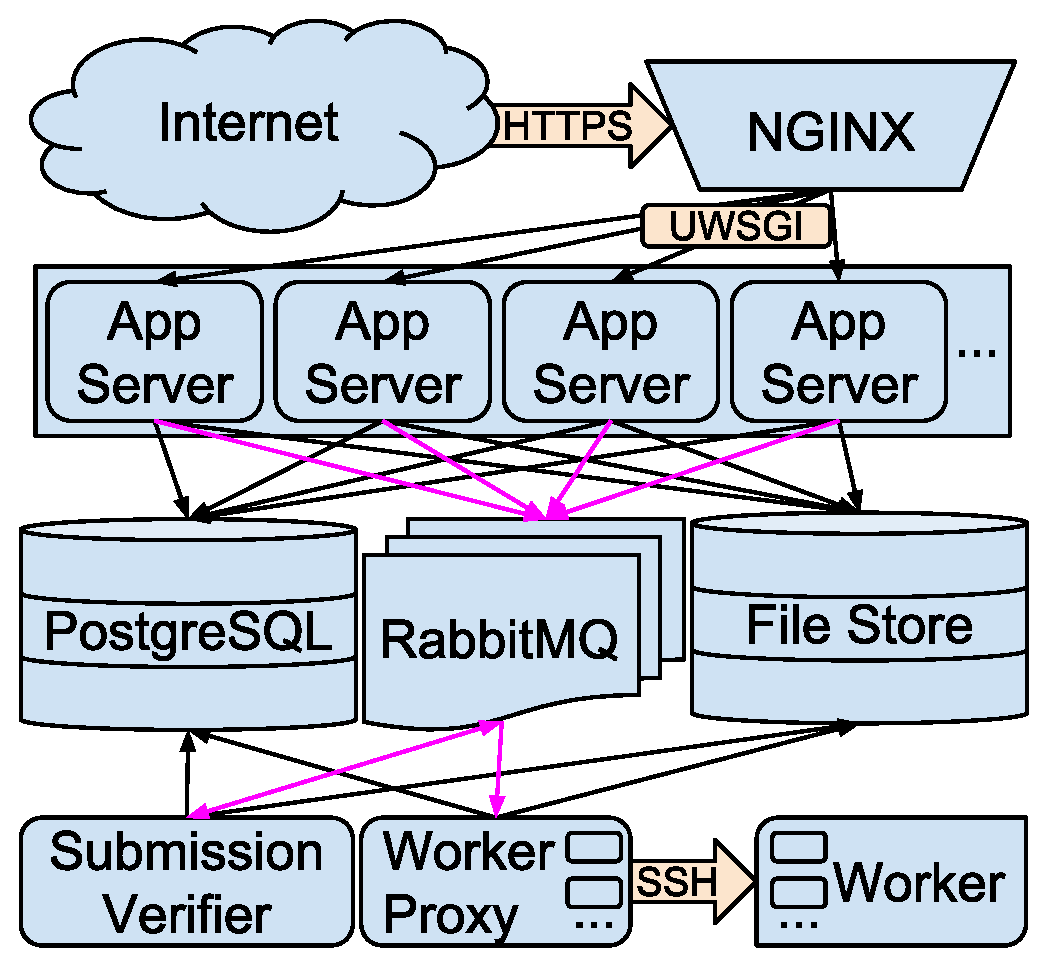
\includegraphics[width=3.3in]{graphs/architecture.eps}
\caption{Provides an overview of the system architecture and how components
  interact. Pink lines indicate messages being passed to and from the RabbitMQ
  service. Note that each \emph{worker} runs in a separate isolated
  environment.}
\locallabel{fig:architecture}
\end{figure}

In this section we describe why we built a submission system, and provide a
high-level overview of its architecture.

\subsubsection{Why}
While a number of submissions systems were available for use, we chose to
design and build our own system for a number of reasons. First, and foremost,
was for the system to be as easy to adopt into existing curriculum in order to
reduce the barriers to entry for instructors in our department. We specifically
designed our system to match existing submission and assessment work flows.

In a similar vein, the \emph{workers} that execute student code needed to run
on existing lab machines in order to provide a consistent test and development
environment without requiring additional resources from our technical support
department. Having consistency further minimized the barriers to entry for
instructors. Additionally, by utilizing existing machines we were able to
provide significant \emph{worker} redundancy permitting us to have zero issues
with the most volatile part of the system at no additional cost to our
department.\footnote{A redesign and implementation of this component was
  required in order to achieve this result. The system has since run with a
  peak activity for three months without a single issue.}

Finally, by building our own system we could ensure having total knowledge of
the entire system. This knowledge allowed us to easily adjust and control the
various aspects of the submission and feedback cycle as necessary for our
research and will allow us to do the same for future research.

In designing the system we had two primary goals:

\begin{itemize}
\item Students should be able to make submissions to their assignments with
  little or no instruction from both the web interface and via the lab machine
  terminals.
\item Reduce the overall assessment time for instructors and their teaching
  assistants.
\end{itemize}

We believe the first goal was met due to a lack of complaints regarding the
usability of the system by the more than 300 students who have used the
system. We confirmed we met the second goal when on more than one occasion an
instructor had to find additional work for their teaching assistants due to a
significant reduction in assessment time. This assessment time includes the
upfront time required to prepare all the test cases for an assignment.


\subsubsection{Architecture Overview}
Figure~\localref{fig:architecture} provides a diagram of the system
architecture. In a nutshell, the primary interface to the system for
instructors, teaching assistants, and students is their web browser, which they
use to access the web interface through the \emph{Internet}. An \emph{NGINX}
web server distributes requests across a number of \emph{app servers} that run
the actual web service code. The system data is stored either in a
\emph{PostgresSQL} database, or deduplicated via an on-disk \emph{file
  store}. A \emph{submission verifier} process exists that checks submissions
for proper files prior to triggering one or more relatively more expensive
build and test jobs. Finally, a one-to-one mapping exists between a
\emph{worker proxy} and a \emph{worker} where the \emph{worker proxy} is
responsible for selecting a machine for the \emph{worker} to run on, initiating
the build and test process, and comparing the generated results to the
assignment's expected results. \emph{RabbitMQ} is used to pass messages that
trigger the jobs run by \emph{submission verifier} and the \emph{worker
  proxies}.

All of the components save for each \emph{worker} run on a single machine as we
have not run into any web service related performance issues. While there is a
single point of failure at that machine, a manual failover to the development
machine requires only minutes, with at worst an hour of data loss. Moreover,
providing redundancy on these components is trivial because the system was
designed to support this expansion pending available hardware.

In addition to the primary web interface, any number of additional interfaces
can be created that work through the system's REST API. For instance, two such
interfaces exist which simplify two distinct tasks for the command-line savvy
users of the system:

\begin{itemize}
\item A submission creation program was written, which authorizes the student
  and creates a submission by first uploading the submission files. The student
  is immediately provided a link where they can view the feedback. This program
  was written to provide transparency with the previous submission process.
\item An assignment test case synchronization program was written, which allows
  an instructor or teaching assistant to quickly synchronize an assignment on
  the system with the contents of a directory on their local system. This
  program dramatically decrease the time to configure and an assignment
  because, while it is easy to add test cases through the web interface, it can
  be tedious if there are more than a handful of them.
\end{itemize}
